\chapter{Background}

This chapter introduces the necessary concepts... %
\autoref{sec:mc} describes... %

\todoZs{Summarize bg}

\section{Model Checking}\label{sec:mc}
% verification
% model checking - what it "promises"
% input model (examples)
% specification or property (examples)
% how does it do that (state space traversal)
% how many executions, what generates these (examples - input is a good one)
% what is the problem (state space explosion)
% what is the state of the art (what are people researching - different techniques, etc. - or whatever you know about this)

% each point is mostly at least a separate paragraph, at most it's own subsection
% use % and go one by one

The challenge of verifying programs without executing or deploying them has been a central research topic since the late 20th century. One of the principal approaches addressing this problem is formal verification, which seeks to provide mathematically rigorous proofs of program correctness.~\cite{MC} %
One of the most used method is model checking~\cite{modelChecking}\cite{modelChecking2} which systematically explores the possible states of a system to determine whether it satisfies a given property. Unlike testing, which examines only a subset of possible behaviors, model checking promises exhaustive verification. %
The model checking problem is an instance of the verification problem. Model checking provides an automated method for verifying concurrent (nominally) finite state systems that uses an efficient and flexible graph search, to determine whether or not the ongoing behavior described by a temporal property holds of the system's state graph.




Model checking~\cite{modelChecking} is a crucial concept when it comes to hardware and software verification as it gives the basis for all possible solutions\todoZs{I don't understand this sentence}. %
It is a widely used method for formal software verification \todoZs{wrong grammar} which main aim is to provide a mathematically precise proof for the correctness of a program. %
By exhaustively traversing through every possible execution of the program for every possible input, it checks whether a certain property was satisfied. %
The main property during this paper was reachability, which means we explore the state space of a program to see if a certain bad state can be reached.

\begin{figure}
  \centering
  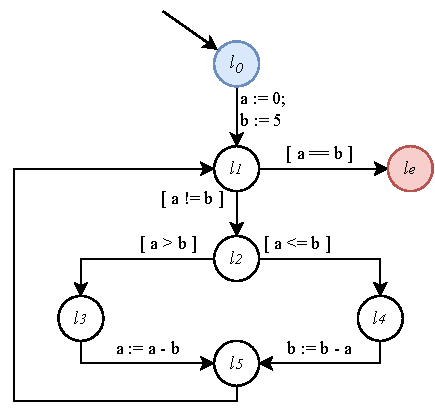
\includegraphics[width=0.5\textwidth]{figures/cfa_simple.drawio.pdf}
  \caption{Simple representation of a Control-Flow Automata (CFA). \todoZs{text on fig is waay too small; if you switch the font to some kind of serif in draw io, it blends in better; also try to create a more wide layout, so it does not take up this much space; empty edges?}}
  \label{fig:cfa}
\end{figure}

\todoZs{again, you can be more verbose and structured, see latex comments}
% possible structure, as a continuation of the above structure:

% input models have to be transformed to an unambiguous and simpler formal representation to reason on
% few (high-level) examples (transition systems, automata)
% common one, originally for software, but widely utilized: CFA
% formal definition of CFA - see Ákos thesis, rephrase it a little, only add what you understand
% and then explain the formal definition shortly, with your own words (similar to what you already did below)

To perform model checking, the program code needs to be represented in a way that makes its control and data flow analyzable. A widely used formalism is the \textbf{Control-Flow Automata (CFA)}~\cite{cfa}. Figure~\ref{fig:cfa} illustrates a simplified CFA, which models how control moves between different parts of a program.

A CFA is a graph-based \todoZs{technically automata-based is more precise, and then I would say "A CFA is an automata, which", or something like that} representation of the program and consists of:
\begin{itemize}
  \item \textbf{Locations} — These represent program points (e.g., line numbers or steps) and are shown as circles in the figure. The blue circle denotes the \textit{initial state}, and the red circle marks the \textit{error state}.
  \item \textbf{Edges} — These indicate transitions between locations and represent operations such as assignments or conditional checks. In the figure, they are visualized as arrows.
\end{itemize}

It helps in analyzing programs\todoZs{what does "helps" mean? instead see above structure - formal representation part}, especially for checking if errors (like reaching a bad state\todoZs{no idea what a bad state is at this point - add a more trivial/everyday example}) can happen. In this documentation\todoZs{report}, I will describe how a BTOR2 program can be transformed into a CFA, and how this representation supports effective model checking\todoZs{I'd rather put a ref to the specific transformation chapter (or for now a placeholder ref)}.

\section{\todoZs{The Hardware Model Checking Format} BTOR2 \todoZs{(or something like that - always go back to section title after section is more or less written and think about what else the title should specify)}}

\todoZs{again, structure, see latex comments}
% hardware model checking: what is this domain, what are we checking; it is a long existing application domain with many successes (cite BMC paper)
% what is a sequential circuit in general terms 

% Btor2: 
% what is it (and maybe try to explain in 1-2 sentences what all the words in it's description mean)
% AIGER successor
% HWMCC: what is HWMCC; it uses btor2 as official format
% btor2 example
% add a subsection on sorts, and maybe mention that we will focus on bitvectors only in this work

The Hardware Model Checking Competition (HWMCC)~\cite{hwmcc} serves as a benchmark for evaluating formal verification tools for hardware systems. A key innovation supporting this effort is BTOR2~\cite{btor2}, a word-level model checking format designed for bit-precise modeling of word-level sequential circuits.
The BTOR2 language extends the previous bit-level AIGER~\cite{AIGER} format with higher-level abstractions, making it ideal for various verification techniques. It introduces a simple, sorted, line-based syntax that is easy to parse and aligns with SMT-LIB~\cite{SMT-LIB} semantics for bit-vectors and arrays.

\todoZs{use more subs(sub)sections - e.g., here you could add "Count2 Example" as a subsection or something - also, it is called count 2, but it is 3 bit, you should clarify why}

\definecolor{backcolour}{rgb}{0.95,0.95,0.92}

\lstdefinestyle{mystyle}{
  backgroundcolor=\color{backcolour}, 
  basicstyle=\ttfamily\footnotesize,
  breakatwhitespace=false,         
  breaklines=true,                 
  captionpos=b,                    
  keepspaces=true,                 
  numbers=left,                    
  numbersep=5pt,
  numberstyle=\ttfamily\footnotesize, 
  frame=none,                                       
  showspaces=false,                
  showstringspaces=false,
  showtabs=false,                  
  tabsize=2
}

\lstset{style=mystyle}
\begin{lstlisting}[language=Verilog, caption=BTOR2 example]
; source: https://github.com/Boolector/btor2tools/tree/b8456dda4780789e882f5791eb486f295ade4da4/examples/btorsim
1 sort bitvec 3
2 zero 1
3 state 1
4 init 1 3 2
5 one 1
6 add 1 3 5
7 next 1 3 6
8 ones 1
9 sort bitvec 1
10 eq 9 3 8
11 bad 10
\end{lstlisting}


In Figure~\ref{fig:count2}\todoZs{use autoref? tell me to help with it} is a BTOR2 circuit that defines a simple finite state machine -- a 3-bit counter -- that starts from zero and increments by one at each time step. Each line defines a node in the circuit, such as a constant, state, operation, or property.

\todoZs{specify that 1,2,... are not the lines, but the node ids (and be consistent with this later)}

\todoZs{I would put this whole thing into a description (\url{https://www.overleaf.com/learn/latex/Lists\#The\_description\_environment}), where each label is "Node x" or something like that - whatever looks good and makes sense}

At the beginning of the circuit, line 1 declares a bit-vector of width 3 \verb|sort bitvec 3|, which serves as the type for all 3-bit values used throughout the circuit. This will have a sort id or \verb|sid| of '1' which will be used to declare registers and operations.

Line 2 defines a constant zero \verb|zero 1|, which produces the bit-vector \verb|000| and has a node id or \verb|nid| of '2'. Following this, line 3 introduces a state variable of sort 1 (3 bits), representing the main state of the circuit.

The initial value of state '3' is specified in line 4, which uses the init keyword to bind state 3 to start at constant 2, which is the \verb|000| bit-vector. The next input is defined in line 5 using one 1, which denotes the constant \verb|001|.

Line 6 defines an addition operation that adds 1 to the main state, resulting in node 6, the next value of the counter. This operation wraps around on overflow due to the fixed 3-bit width. Line 7 then uses the next keyword to specify that in the next state, the counter should take the value of node 6, i.e., the incremented result.

To define a property of interest, line 8 declares another constant: \verb|ones 1|, which represents the maximum value a 3-bit counter can hold—namely \verb|111|. Line 9 introduces a new sort of width 1, which is used for boolean-like signals such as equality checks.

Line 10 defines a comparison between the current counter value and the maximum value \verb|111| using the eq operator. This operation returns a 1-bit result: true (1) if the counter is at maximum, false (0) otherwise. Finally, line 11 marks this equality result as a bad state, which is a safety property violation. Hence, the circuit asserts that reaching the value 111 is undesirable or erroneous.

\todoZs{I'll go through the description of the example when it's made into a description}

In summary, this BTOR2 circuit models a 3-bit counter that increments with each step and triggers a bad state when it reaches 111. This design could be used in formal verification to prove that the system avoids overflow, or alternatively, to find the point at which it does. The clear structure and modular nature of BTOR2 make it suitable for such sequential hardware modeling and property checking.

\subsection{Btor2C}

\todoZs{structure in latex comments}
% what is Btor2C, what does it do
% why is it useful (in a bit more detail? see abstract, I think we talked about this more there, maybe not in the final version, idk)
% an example of a C program from a btor2 circuit (C can be simplified, just mention that)

Btor2C~\cite{btor2c} is a tool that translates Btor2 hardware models into equivalent C programs. This allows software verification tools to analyze hardware designs, bridging the gap between hardware and software verification.
\todoZs{you don't need to talk about your work yet - the reader has no idea what your implementation is yet anyways - but that's for later} In my implementation, I focused on bit-vectors and their related functions and definitions, leveraging the expressive power of BTOR2 to model and verify small, bit-precise sequential systems.

\todoZs{So far it was clear what we need to introduce - but jumping to Theta next seems to make a hole here to me - we will need to think about what else needs to be introduced - but maybe do that while starting to write the next chapter(s) - I think a lot of stuff will come up}

\section{Theta}

Regarding the implementation\todoZs{the what? just introduce theta, this is not the place to talk about you using it :D}, I chose Theta~\cite{theta}, a modular and extensible model checking framework developed by the Critical Systems Research Group at the Budapest University of Technology and Economics, as the target platform for integrating a BTOR2 frontend.

\todoZs{What I'm missing from the introduction are the existing frontends}

To begin, I defined an unofficial BTOR2 grammar using ANTLR4~\cite{antlr}, a powerful parser generator widely adopted in both academia and industry for constructing interpreters, compilers, and domain-specific languages.

Theta supports abstraction-refinement based reachability analysis. In my project, I worked with XCFA models—an extension of Control Flow Automata (CFA) that incorporates procedures and concurrency - but focused primarily on the CFA subset. This allowed me to apply Theta's robust CEGAR-based algorithms for reachability checking.

\todoZs{for now, after the above fixes, I would leave the bg a bit, but keep an open eye when writing the next things for any element that needs to be introduced and add todos here for each of them}